\documentclass{article}
\usepackage{graphicx}
\usepackage{amsmath}
\usepackage{cite}
\usepackage{color}
\usepackage{enumitem}
\usepackage{hyperref}
\usepackage{natbib}
\usepackage{tabularx}
\usepackage{natbib}
\usepackage{ragged2e}

\title{\textbf{"Principi di Reti Neurali"}}
\author{Alessandro Meloni GEPID}
\date{}
\begin{document}
\maketitle
\begin{abstract}
\begin{justify}
    Questo paper si soffermerà sull'analisi, la nascita, l'evoluzione delle reti neurali e i principi del loro funzionamento. Il punto focale sarà sicuramente quello di capire quanto un'intelligenza artificiale di questa portata, possa influire sul lavoro e la relativa organizzazione.In relazione a ciò, comprendere finquanto esse si possano spingere, quanta concorrenza potrebbero generare e i risvolti positivi/negativi sulla domanda di lavoro.
\end{justify}
\end{abstract}
\centering \tableofcontents
\centering \newpage
\section{Le Reti neurali}
\flushleft \subsection{Cosa sono?}
\citep{IBM2021}
\flushleft\subsection{Quando sono state istituite?}

\centering \newpage
\section{Il funzionamento}

 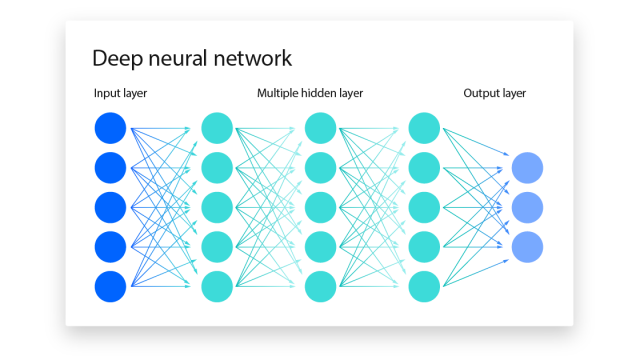
\includegraphics[width = 0.5\linewidth]{PROGETTO RETI NEURALI/ImmaginiProgetto/NeuNet.jpg}
    \label{F1:foto reti}

\flushleft \subsection{Come si comportano?}

\flushleft \subsection{A cosa servono?}
 
\flushleft \subsection{L'organizzazione e il mercato del lavoro}

\centering \newpage
\section{Considerazioni finali}
\bibliography{Database}
\bibliographystyle{plainnat}
\end{document}
